% !TeX spellcheck = fr_FR
\chapter{Chapitre 2 : Algorithmes}

Ce chapitre concerne les différents algorithmes de traitement des données du chapitre 1.

\section{Filtrage de données LIDAR}

L'utilité de réduire la quantité de données sauvegardées de nos jours au vu des moyens de stockage moderne employé n'est plus une occupation majeure.
Cependant, certains systèmes restent limités en cette ressource.
Le filtrage des données \gls{lidar} reste toutefois utile sur des systèmes plus puissants pour accélérer l'utilisation ultérieure des fichiers. Les méthodes présentées ici peuvent être utilisées indépendamment ou bien combinées.

\subsection{Filtre par classe de point}
Une première méthode pour filtrer les données est de se baser sur la classification des points du chapitre 1.1. En connaissant les informations qui nous intéressent, le filtrage se fait donc lors de la lecture des données.
Étant données que la lecture se déroule de manière séquentielle, il suffit de poser une ou plusieurs conditions vérifiant la classe du point.
Si la condition est respectée, le point est collecté dans une liste de points à garder, le cas échéant étant simplement de l'ignorer.
Une fois la lecture terminée, on réécrit la liste des points gardés dans un nouveau fichier \gls{lidar}.
Le fichier original peut être supprimé ou conservé.

\subsection{Filtre par point pondérer}

Une autre manière de réduire la quantité de données est de remplacer plusieurs points par un seul où l'élévation de celui-ci équivaut à la moyenne des élévations des voisins.
En d'autres termes $$ P_{\bar{y}} = \frac{1}{n} \sum_{i=0}^{n} p_{iy} $$
où $n$ est le nombre de voisins d'un point $P$. 
Le choix de l'endroit où l'on créera le point peut être déterminé à l'aide d'une condition, p. ex. $$\sum_{i=0}^n dist(P, p_i) \geq \epsilon$$

Un effet de bord de cette méthode est le lissage des surfaces plates. Un exemple serait les illustrations \ref{fig:before_las_filter} et \ref{fig:after_las_filter} où l'on peut observer qu'après une reconstruction de surface, on aperçoit que les points on une tendance à moins osciller dans l'axe vertical.

\begin{figure}[tbh!]
    \centering
    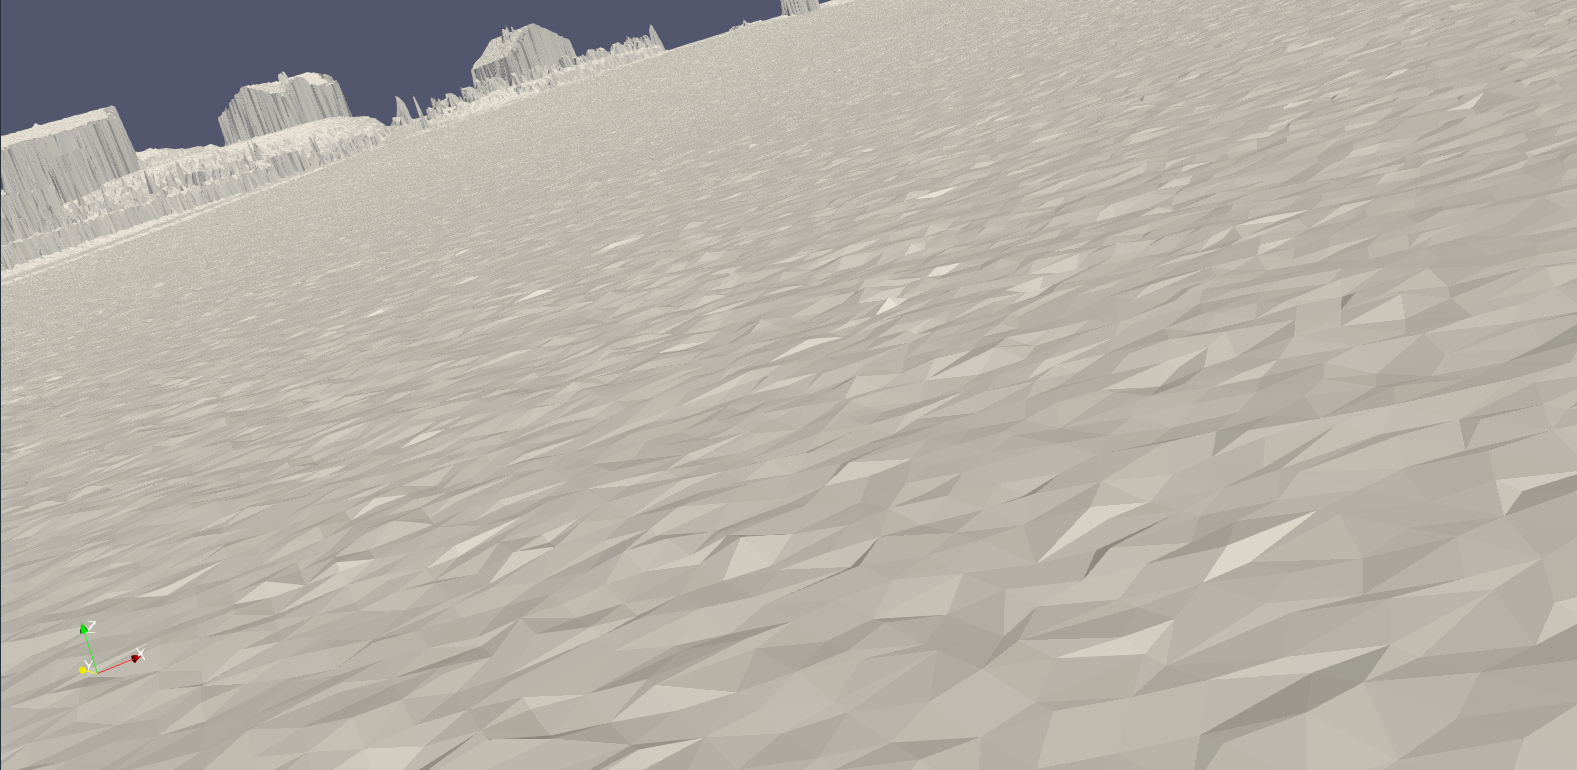
\includegraphics[width=0.8\linewidth]{figures/lissage_brut.png}
    \caption{Surface plane avant le passage par un filtre. Source : réaliser par Jérôme Chételat}
    \label{fig:before_las_filter}
\end{figure}
\begin{figure}[tbh!]
    \centering
    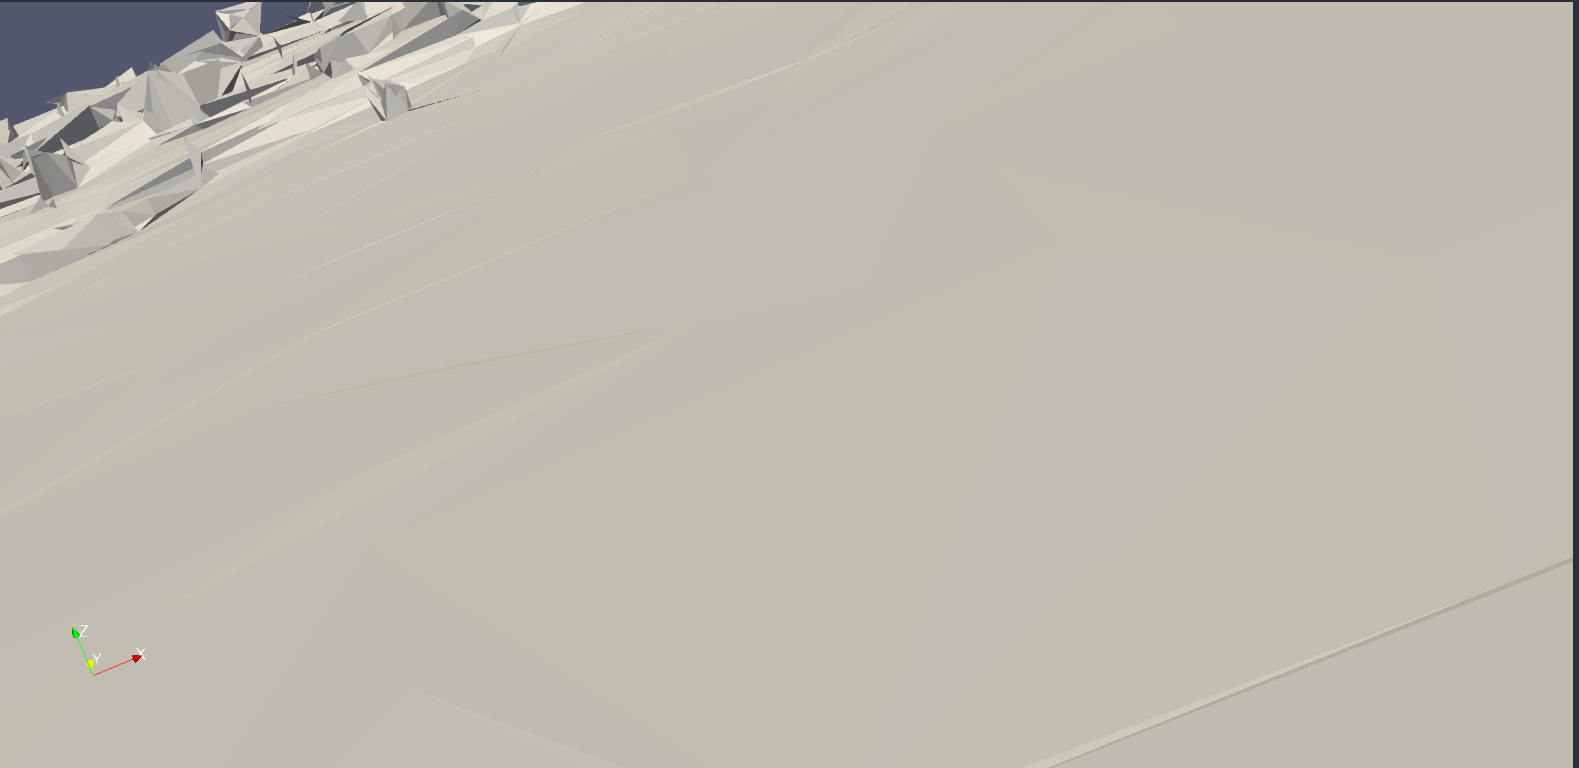
\includegraphics[width=0.8\linewidth]{figures/lissage_filtrer.png}
    \caption{Surface plane après le passage par un filtre. Source : réaliser par Jérôme Chételat}
    \label{fig:after_las_filter}
\end{figure}
\section{Triangulation de Delaunay}

La triangulation de Delaunay est une manière de créer des triangles entre des points dispersés dans l’espace.
Cette manière de trianguler les points permet de créer un résultat plus homogène que d’autres méthodes.

\begin{figure}[htb!]
    \centering
    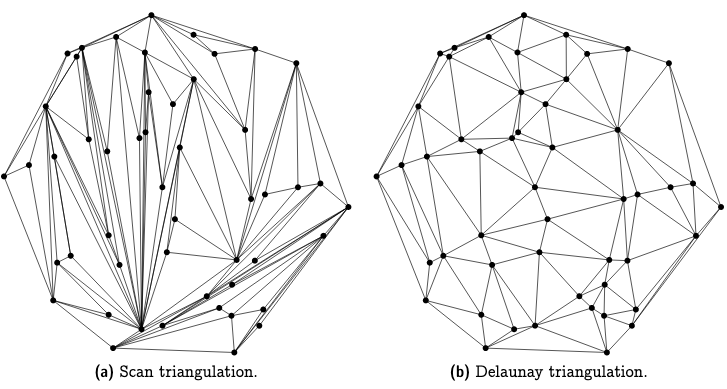
\includegraphics[width=0.8\linewidth]{figures/triangulation-example.png}
    \caption{Deux triangulations du même jeu de données. Source : tiré de ref URL01}
    \label{fig:triangulation_example}
\end{figure}

\subsection{Principe de l'algorithme}
Il existe plusieurs algorithmes pour recréer des triangles entre des points.
Il s’agit de l’algorithme de Bowyer-Watson, un algorithme itératif découvert par Adrian Bowyer et David Watson.
Le principe de ce procédé se repose sur l’ajout progressif de points dans la triangulation.
Après chaque ajout, de nouveaux triangles sont formés à partir du point ajouté et des sommets du triangle contenant le point.

\subsection{Déroulement de l'algorithme}
Soit $\mathcal{P} \subset \mathbb{R}^2$ l'ensemble des points à trianguler et $\mathcal{T}$ les triangles appartenant à la triangulation. On construit dans un premier temps, un triangle $S \in \mathcal{T}$ tel que $\mathcal{P} \subset S$. On nomme ce triangle le "super-triangle". Il doit contenir en son sein l'ensemble de points $\mathcal{P}$. On ajoute donc trois points, les sommets de $S$ dans $\mathcal{P}$.

On prend ensuite un point de $\mathcal{P}$ puis on détermine dans quel triangle il se situe.
Pour connaître l'appartenance d'un point à un triangle, on détermine si un point est contenu dans le cercle circonscrit d'un triangle.
La condition qui permet de déterminer si un point $D$ est contenu dans le cercle-circonscris de $\triangle ABC$ est la suivante :

$$
\begin{vmatrix}
 A_x - D_x & A_y - D_y & (A_x - D_x)^2 + (A_y - D_y)^2 \\
 B_x - D_x & B_y - D_y & (B_x - D_x)^2 + (B_y - D_y)^2 \\
 C_x - D_x & C_y - D_y & (C_x - D_x)^2 + (C_y - D_y)^2 \\
\end{vmatrix} \geqslant 0
$$

Si la condition est vraie, le point est relié au sommet du triangle qui le contient. Les triangles formés désormais appartiennent à $\mathcal{T}$.

On répète les opérations d'ajout de points et de création de triangles jusqu'à ce qu'on ait parcouru tous les points de $P$

Pour finir, on supprime les sommets du super-triangle ainsi que ses arrêtes de $\mathcal{P}$ et de $\mathcal{T}$.

Le résultat est un ensemble de triangles $\mathcal{T}$ représentant des surfaces appelées triangulation de Delaunay.
Ce résultat est unique pour un ensemble de points $\mathcal{P}$ donné.
En voici un exemple ci-dessous.

\section{Fusion de maillage}

L'algorithme présenté dans cette section concerne la fusion de maillage. Dans l'application du travail de bachelor, il se peut que l'on ait déjà des triangulations existantes et que l'on souhaite afficher un résultat de la fusion des deux triangulations. Il s'agit en réalité qu'une partie d'un autre algorithme de triangulation basé sur le principe de "Divide and conquer".

\subsection{Principe de l'algorithme}

